\documentclass[]{article}

\usepackage[margin=1.0in]{geometry}

% Figures
\usepackage{graphicx}
\graphicspath{{figures/}}

% Trick Latex into placing all figures and tables at the end of the document
% regardless of their position in the source code.
\renewcommand{\textfraction}{1.0}
\renewcommand{\floatpagefraction}{0.9}

% Equations
\usepackage{amsmath}

% Bibliography
\usepackage{natbib}

% Better tables
\usepackage{booktabs}
\usepackage{multirow}
\newcommand{\ra}[1]{\renewcommand{\arraystretch}{#1}}


%--------------------------------------------------
% TITLE
%--------------------------------------------------
\title{SIO 217A: Cloud Droplet Growth}
\author{Team MecheE \\ Bengu Ozge Akyurek, David Larson, Guangchao Wang}
\date{\today}

\begin{document}

\maketitle


%--------------------------------------------------
% INTRO
%--------------------------------------------------
\section{Introduction}
Brief summary of how the topic affects atmospheric thermodynamics.


%--------------------------------------------------
% MODEL
%--------------------------------------------------
\section{Cloud Droplet Growth}

\subsection{Model Description}
Description of the model, its assumptions, and its possible shortcomings.


The growth rate of a droplet by diffusion can be approximated as
\begin{align}
    \label{eq:5.26}
    r \frac{dr}{dt} = (S - 1) \left[ \frac{L_{lv}^2 \rho_l}{\kappa R_v T^2} + \frac{\rho_l R_v T}{e_s(T) D_v} \right] ^{-1} = \frac{S - 1}{K + D}
\end{align}
where $K$ and $D$ are the thermodynamic terms associated with heat conduction
and diffusion of water vapor, respectively.

Assuming the atmospheric ambient conditions are constant (i.e. $S$, $K$, and
$D$ are constant), then Equation~\ref{eq:5.26} can be integrated to get
\begin{align}
    \label{eq:5.27}
    r(t) = \left[ r_0^2 + \frac{2(S -1)}{K + D}(t - t_0)^2 \right] ^{1/2},
\end{align}
which can then be rearranged to find $t$

\begin{align}
    t = (r^2 - r_0^2) \frac{K + D}{2(S - 1)}
\end{align}

Using the values from Table~\ref{tab:parameters}


\begin{table}[h]
    \centering
    \caption{Paramters for droplet growth rate.}
    \label{tab:parameters}

    \begin{tabular}{l l l l}
    \toprule
    Parameter & Value & Units & Notes\\
    \midrule
    $S - 1$   & 0.05            & \%                         & \\
    $p$       & 900             & $mb$                       & \\
    $T$       & 273             & $K$                        & \\
    $r_0$     & 0.75            & $\mu m$                    & \\
    $L_{lv}$  & 2.5x10$^{6}$    & $J \ kg^{-1}$              & pure water at $T=273 K$ \\
    $\rho_l$  & 1000            & $kg \ m^{-3}$              & pure water at $T=273 K$ \\
    $R_v$     & 461             & $J \ kg^{-1} K^{-1}$       & \\
    $\kappa$  & 2.4x10$^{-2}$   & $J \ m^{-1} s^{-1} K^{-1}$ & $T=273 K$ \\
    $D_v$     & 2.21x10$^{-5}$  & $m^2 s^{-1}$               & $T=273 K$, $p=1000 mb$ \\
              & 2.46x10$^{-5}$  & $m^2 s^{-1}$               & $T=273 K$, $p=900 mb$ \\
    $e_s (T)$ & 6.15            & $mb$                       & $T=273 K$\\
    \bottomrule
    \end{tabular}
\end{table}


\begin{table}[h]
    \centering
    \caption{Growth rate of droplets with nuclei of NaCl, ($S - 1$)=0.05\%,
        $p$=900mb, $T$=273K, and $r_0$=0.75$\mu$m recreated from Table 5.5 of \cite{Curry}.}

    \ra{1.2}
    \begin{tabular}{@{} c r r r @{}}
        \\
        \toprule
        m [g] & $10^{-14}$ & $10^{-13}$ & $10^{-12}$ \\
        \midrule
        r [$\mu$m] & \multicolumn{3}{c}{t [s]} \\
        \midrule
        1  & 2.4    & 0.15   & 0.013 \\
        2  & 130    & 7.0    & 0.61 \\
        4  & 1,000  & 320    & 62 \\
        10 & 2,700  & 1,800  & 870 \\
        20 & 8,500  & 7,400  & 5,900 \\
        30 & 17,500 & 16,000 & 14,500 \\
        50 & 44,500 & 43,500 & 41,500 \\
        \bottomrule
    \end{tabular}
\end{table}


\subsection{Model Parameters}
Physical significance of the model parameters you are calculating and varying.


%--------------------------------------------------
% RESULTS
%--------------------------------------------------
\section{Results of Modeling Study}
Conclusions you draw from your modeling study, with as much physical insight
as the modeling results allow.

\begin{figure}
    \centering
    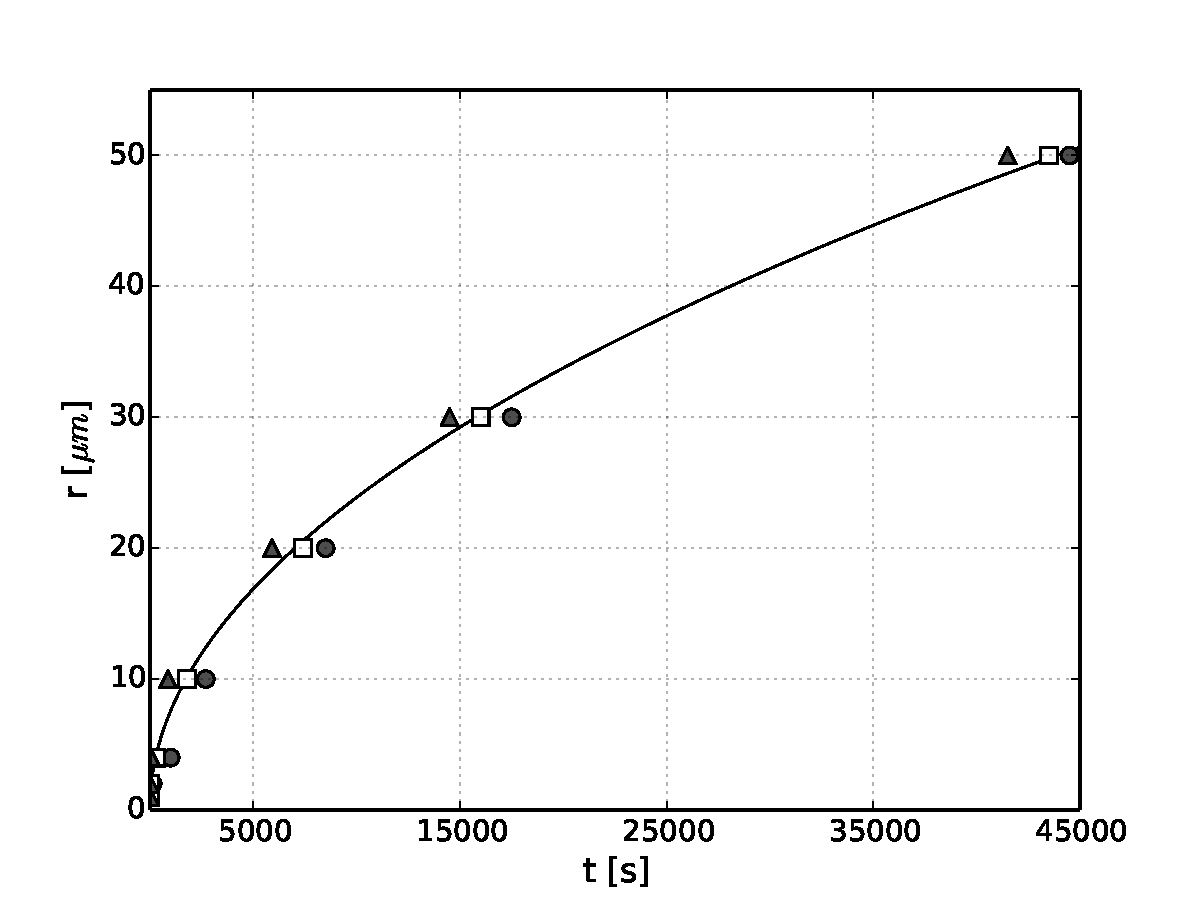
\includegraphics[width=\textwidth]{r_t.pdf}
    \caption{Droplet growth rate ignoring curvature and solute effects. The solid black line is the model, while the solid gray triangle, black outlined square, and solid gray circle are the radiuses from Table 5.5 of \cite{Curry} for $m_{solt}$ = 10$^{-12}$, 10$^{-13}$, and 10$^{-14}$ [g], respectively.}
\end{figure}

\begin{figure}
    \centering
    \caption{Droplet growth rate for varying ambient temperatures.}
\end{figure}

\begin{figure}
    \centering
    \caption{Droplet growth rate for varying supersaturation value.}
\end{figure}


%--------------------------------------------------
% CONCLUSION
%--------------------------------------------------
\section{Conclusion}


%--------------------------------------------------
% BIBLIOGRAPHY
%--------------------------------------------------
\bibliography{sources}
\bibliographystyle{plainnat}


\end{document}
